\lecture{19}{Wed 14 Feb '24}{}
We will now prove the \nameref{thm:cauchy-binet}.
\begin{lemma*}[Sylvester's determinant identity] \label{thm:sylvester}
    Let $A \in \R^{n \times m}$ and $B \in \R^{m \times n}$.
    Then \[
        \lambda^m \det(\lambda I_n + AB) = \lambda^n \det(\lambda I_m + BA).
    \]
\end{lemma*}
\begin{proof}
    Use $2\times 2$ block matrices.
    Note that \begin{align*}
        \begin{pmatrix}
            \lambda I_n & A \\
            B & \lambda I_m
        \end{pmatrix}
        &= \begin{pmatrix}
            I_n & 0 \\
            B & I_m
        \end{pmatrix} \begin{pmatrix}
            \lambda I_n & 0 \\
            0 & \lambda I_m - BA
        \end{pmatrix} \begin{pmatrix}
            I_n & A \\
            0 & I_m
        \end{pmatrix} \\
        &= \begin{pmatrix}
            I_n & A \\
            0 & I_m
        \end{pmatrix} \begin{pmatrix}
            \lambda I_n - AB & 0 \\
            B & \lambda I_m
        \end{pmatrix} \begin{pmatrix}
            I_n & 0 \\
            B & I_m
        \end{pmatrix}.
    \end{align*}
    \begin{fact}
        For such block matrices, the determinant of an upper or lower
        triangular block matrix is the product of the determinants of the
        diagonal blocks.
    \end{fact}
    Then we have \begin{align*}
        \det\begin{pmatrix}
            \lambda I_n & A \\
            B & \lambda I_m
        \end{pmatrix}
        &= \lambda^n 
    \end{align*}
\end{proof}
\begin{proof}[Proof of Cauchy-Binet]
    Compare the coefficient of $\lambda^{m-n}$ in the two sides of \[
        \lambda^{m-n} \det(\lambda I_n + AB) = \det(\lambda I_m + BA).
    \]
\end{proof}

\section{Planar Graphs} \label{sec:planar_graphs}
\begin{definition}[Planar graph] \label{def:planar_graph}
    A graph which can be drawn in the plane without edges intersecting in
    non-vertices is called a \emph{planar graph}.
    We can allow loops and parallel edges.

    A planar graph together with its planar embedding is called a
    \emph{plane graph}.
\end{definition}
\begin{examples}
    \item \leavevmode\begin{center}
        $\vcenter{\hbox{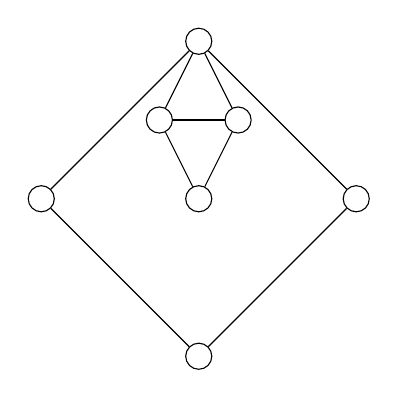
\begin{tikzpicture}
            \node[draw,circle] (a) at (0,0) {};
            \node[draw,circle] (b) at (-2, -2) {};
            \node[draw,circle] (c) at (0, -4) {};
            \node[draw,circle] (d) at (2, -2) {};
            \node[draw,circle] (e) at (-0.5, -1) {};
            \node[draw,circle] (f) at (0, -2) {};
            \node[draw,circle] (g) at (0.5, -1) {};
            \draw (a) -- (b) -- (c) -- (d) -- (a);
            \draw (a) -- (e) -- (f) -- (g) -- (a);
            \draw (e) -- (g);
        \end{tikzpicture}}}$ \quad and \quad
        $\vcenter{\hbox{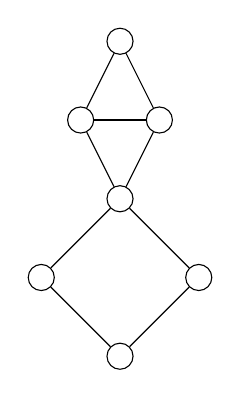
\begin{tikzpicture}
            \node[draw,circle] (a) at (0,0) {};
            \node[draw,circle] (b) at (-1, -1) {};
            \node[draw,circle] (c) at (0, -2) {};
            \node[draw,circle] (d) at (1, -1) {};
            \node[draw,circle] (e) at (-0.5, 1) {};
            \node[draw,circle] (f) at (0, 2) {};
            \node[draw,circle] (g) at (0.5, 1) {};
            \draw (a) -- (b) -- (c) -- (d) -- (a);
            \draw (a) -- (e) -- (f) -- (g) -- (a);
            \draw (e) -- (g);
        \end{tikzpicture}}}$
    \end{center}
    are isomorphic as planar graphs, but not as plane graphs.
    \item Edges need not be straight lines.
    Thus $K_4$ is planar.
    \begin{center}
        \begin{tikzpicture}
            \node[draw,circle] (a) at (0,0) {};
            \node[draw,circle] (b) at (2,0) {};
            \node[draw,circle] (c) at (2,2) {};
            \node[draw,circle] (d) at (0,2) {};
            \draw (a) -- (b) -- (c) -- (d) -- (a);
            \draw (a) -- (c);
            \draw (b) .. controls (0.5, -2) and (-2, 0.5) .. (d);
        \end{tikzpicture}
    \end{center}
\end{examples}
\begin{fact}[Jordan curve theorem] \label{thm:planar_graphs:jordan}
    A plane graph partitions the plane into disjoint regions, which we call
    \emph{faces}.
    We also include the unbounded face.
\end{fact}
\begin{theorem*}[Euler's theorem] \label{thm:planar_graphs:euler}
    Let $G$ be a connected planar graph with $V$ vertices, $E$ edges,
    and $F$ faces.
    Then \[
        V - E + F = 2.
    \]
\end{theorem*}
\begin{proof}
    We induct on $E$.
    If $E = 0$, then $V = 1$ and $F = 1$, so the result holds.
    Suppose the result holds for all connected planar graphs with $E - 1$
    edges.

    We find an edge $e$ such that removing $e$ from $G$ gives a connected
    graph $G'$.
    Removing $e$ will merge the two faces on either side of $e$.
    Then $G'$ has $V$ vertices, $E - 1$ edges and $F - 1$ faces.
    Then $V - E + F = V - (E-1) + (F-1) = 2$.

    If such an edge does not exist, \ie, removing any edge disconnects the
    graph, then $G$ is a tree.
    So $V - E + F = V - (V - 1) + 1 = 2$.
\end{proof}
\begin{remark}
    Planar graphs can also be embedded on a sphere.
\end{remark}

\begin{definition}[Bipartite graph]  \label{def:planar_graphs:bipartite}
    A \emph{bipartite graph} $G = (V, E)$ is one where
    $V = V_1 \sqcup V_2$ such that no edge connects two vertices in the same
    set.
    The \emph{complete bipartite graph} $K_{m,n}$ is the bipartite graph
    where $\abs{V_1} = m$, $\abs{V_2} = n$, and $\set{v_1, v_2} \in E$ for
    all $v_1 \in V_1$ and $v_2 \in V_2$.
\end{definition}
\begin{corollary}
    $K_{3, 3}$ is not planar.
\end{corollary}
\begin{proof}
    Suppose it were.
    $V = 6$, $E = 9$, so by Euler's theorem, $F = 5$.
    But each face must have at least 4 edges since $K_{3, 3}$ is bipartite.
    Summing over all faces, we get $2E \geq 4F$, a contradiction.
\end{proof}

\begin{definition}[Minor] \label{def:planar_graphs:minor}
    A \emph{minor} of a graph $G$ is one obtained by deleting vertices or
    edges, or \emph{contracting} edges.
    An edge is contracted by removing it and merging its two endpoints.
\end{definition}
\begin{fact*}[Kuratowski's theorem] \label{thm:planar_graphs:kuratowski}
    A graph is planar iff it has no minor isomorphic to $K_5$ or $K_{3,3}$.
\end{fact*}

\begin{definition}[Colouring] \label{def:planar_graphs:colouring}
    A \emph{(vertex) colouring} of a graph $G$ is an assignment of colours
    to the vertices of $G$ so that adjacent vertices have different colours.
\end{definition}

\begin{fact*}[Four colour theorm] \label{thm:planar_graphs:4colour}
    Any planar graph can be coloured using at most 4 colours.
\end{fact*}
